% !TEX root = ../main.tex
\newpage
\section{\mywork Mean Field Reductions for undirected graphs}
We will now investigate the questions that were raised after deriving the \MFR. How do we deal with the curse of dimensionality concerning the degree distribution? But there are also other questions to be answered. If the synchronisation dynamics of the network of Theta neurons \eqref{eq:thetaneuronnetwork} can be predicted by the Ott-Antonsen reductions \cref{eq:OttAntonsenSystemFull, eq:OttAntonsenMeanField} and \eqref{eq:MeanField}, then it can also be measured by the order parameter \eqref{eq:orderparameter}. These systems describe the same quantity, but how can we show that?


\subsection{Directed graphs as permutations}
So how can we use the \MFR efficiently when the network is a directed graph with an asymmetrical adjacency matrix? Let's investigate.
\begin{itemize}
\item Sampling $\kinb$ and $\koutb$ from a bivariate distribution requires us to find the marginal distribution of $P$ for $\kinb$, sampling $\kinbi$, and then sampling $\koutbj$ from $P$ while keeping $\kinbi$ fixed. This is a cumbersome process. And what relation would there be between $\kinb$ and $\koutb$?
\item However, if we assume that the marginal distributions for $\kinb$ an $\koutb$ are independent, there is a simplification to be found. We can even assume that the two marginal distributions are identical univariate distributions. 
\item Hence, we can sample $\kinb$ from a univariate distribution and find $\koutb = \permute ( \kinb )$ so that the total number of links remains constant. 
\end{itemize}

This hypothesis can be tested: we assume that $P(\k) = P(\kin) \cdot P(\kout)$ so that $P$ consists of two identical and independent distributions, given by the distributions presented in Chapter \ref{sec:NetworkTopologies}. Then, we sample $\kinb \sim P(\kin)$ and perform a permutation to find all node degrees $\k_j$. The surface given by $P$ and the histogram of $\k_j$ have been plotted in Figure \ref{fig:2Ddistributions}. As we can see, the variates follow the distribution well. 

\begin{figure}[ht]
\centering
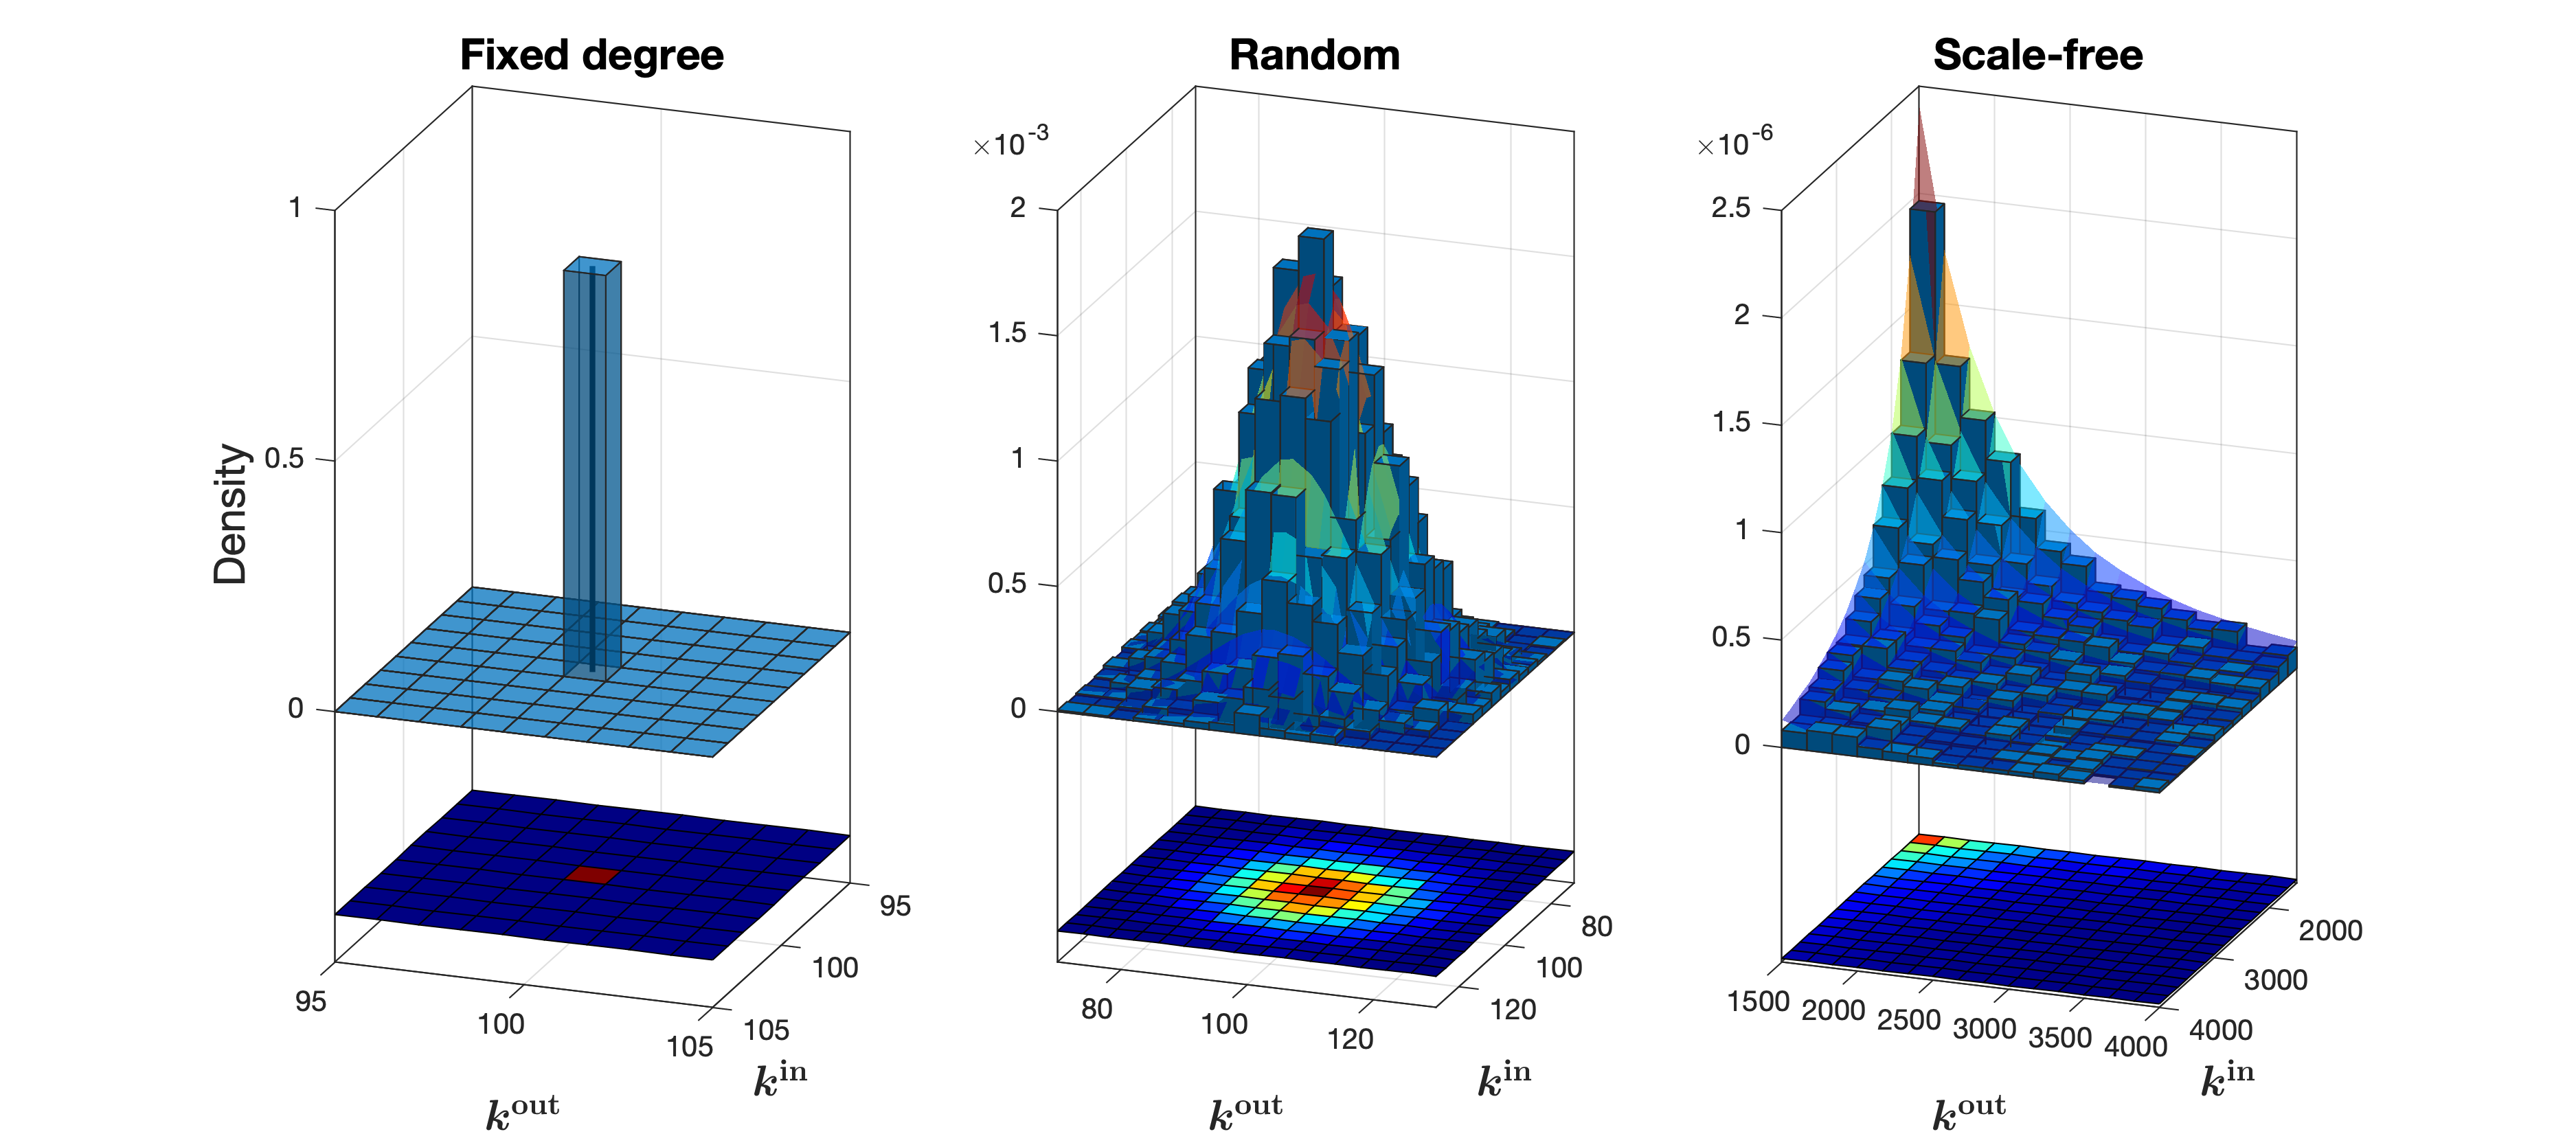
\includegraphics[trim=2.5cm 0cm 2.5cm 0cm, clip=true, width = \textwidth]{../Figures/Distributions/2D.png}
\caption{Bivariate distributions for different network topologies, using 10$^4$ number of samples. The surface given by $P(\k)$ is well approximated by the histogram of variates sampled from a univariate distribution. $\kmean =  2 \times 10^3$ for all topologies, $p \approx 0.2$ for the random network and $\gamma = 4.3$ for the scale-free network.}
\label{fig:2Ddistributions}
\end{figure}
Hence, we can use univariate distributions in our simulations of the Ott-Antonsen Mean Field \eqref{eq:OttAntonsenMeanField}.


\subsection{Building the adjacency matrix} \label{sec:buildingA}
If we want to simulate the network of theta neurons \eqref{eq:thetaneuronnetworkcurrent} we need to construct the adjacency matrix. We can find an exact solution for $A$ given the degree vectors in \eqref{eq:definekinkoutfromP}. $A_{ij}$ represents a directed graph, but $A_{ij} \neq A_{ji}$ is not a necessary condition. For the elements of $A_{ij}$ we need to find $N^2$ number of variables. We have the following constraints:
\begin{enumerate}
\item The column- and row-sums of $A_{ij}$ must be equal to $\kinb$ and $\koutb$, see \eqref{eq:definekinkoutfromA}. 2$N$ constraints.
\item Self-coupling is mandatory: $A_{ii} = \boldsymbol{1}$. $N$ constraints.
\item The total number of links is constant: $\sum_{i=1}^{N} \kinbi \equiv \sum_{j=1}^{N} \koutbj \equiv \sum_{i,j=1}^{N}A_{i j}$. 1 constraint.
\end{enumerate}
This means that there are $N^2 - (3N + 1)$ variables to find. Once a solution has been found, $A_{ij}$ can be switched with element $A_{ic}$ if $A_{ij} \neq A_{ic}$ and $A_{rj}$ with $A_{rc}$, which yields a new feasible solution. The number of switches one can make is high, and therefore we can simply try a stochastic approach to obtain $A$:
\begin{enumerate}
\item Choose a random row $i \in [1,N]$. $A_{i,i} = 1$, so we need $m = \kinbi - 1$ elements that are 1.
\item Perform $\permute ( \koutbj, j \neq i)$ and therein find the indices $\boldsymbol{\ell}$ of the $m$ first largest elements. 
\item Set $A_{il} = 1 \: \: \forall \: \: l \in \permuteinv (\boldsymbol{\ell})$.
\end{enumerate}
Algorithms that find the largest value in a vector start from the first or the last element. The permutation allows us to find different maxima every time by shuffling the vector.

\begin{figure}[ht]
\centering
\begin{subfigure}[b]{0.32\linewidth}
   \centering
  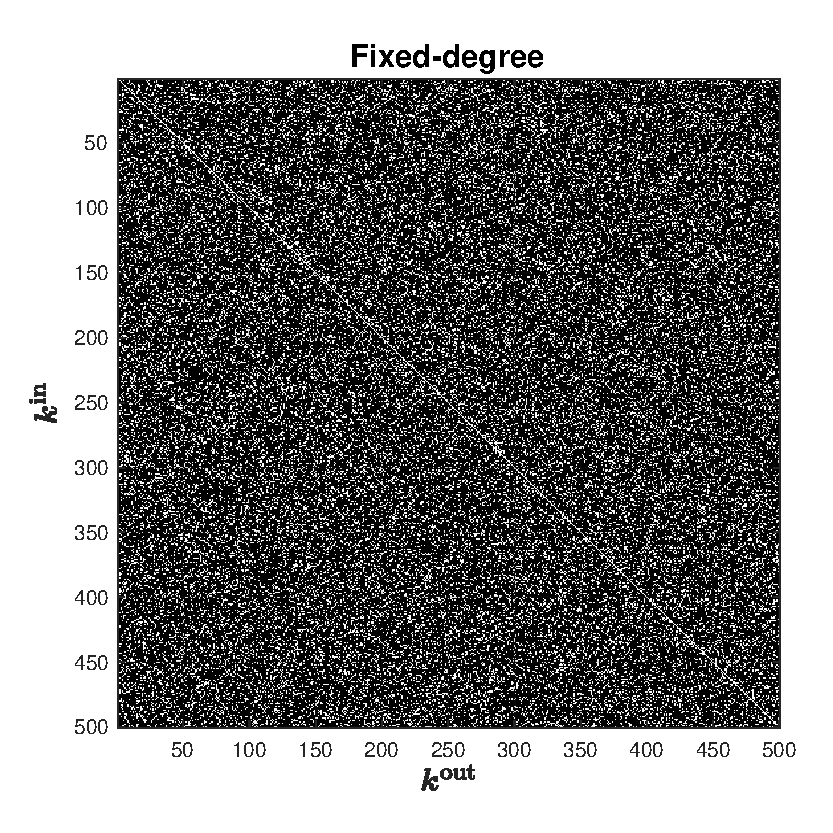
\includegraphics[width=\linewidth, trim={0.5cm 0.5cm 1cm 0.5cm },clip]{../Figures/Adjacency matrices/A_fixeddegree.pdf}
%   \caption{Adjacency matrix for a fixed-degree network.}
 %  \label{fig:A_fixeddegree} 
\end{subfigure} \hfill
\begin{subfigure}[b]{0.32\linewidth}
   \centering
  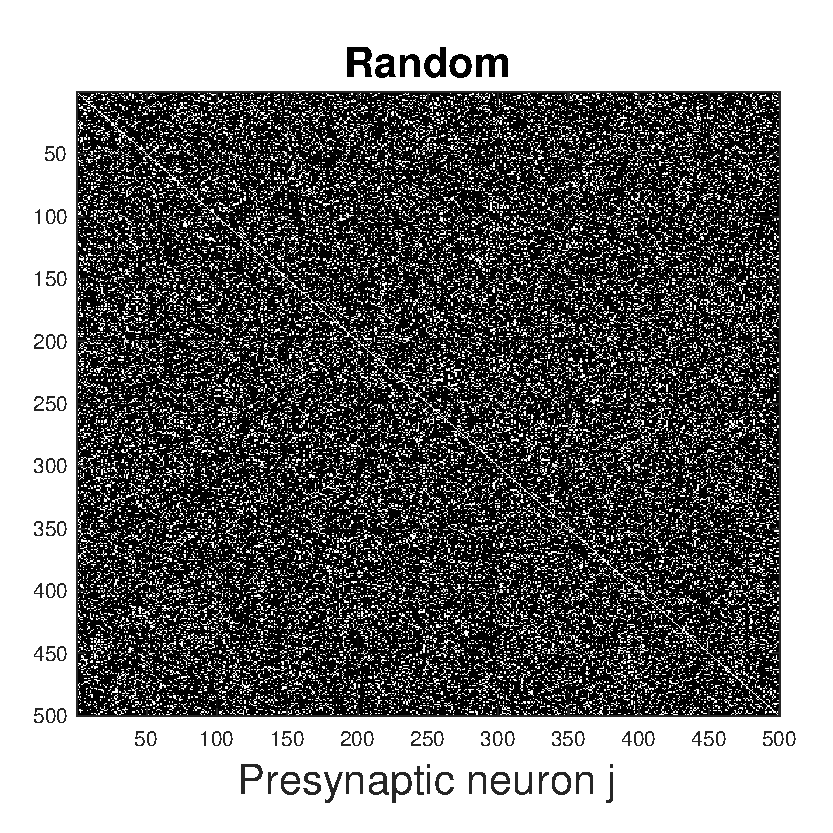
\includegraphics[width=\linewidth, trim={0.5cm 0.5cm 1cm 0.5cm },clip]{../Figures/Adjacency matrices/A_random.pdf}
%   \caption{Adjacency matrix for a fixed-degree network.}
%   \label{fig:MFRPSS}
\end{subfigure} \hfill
\begin{subfigure}[b]{0.32\linewidth}
   \centering
  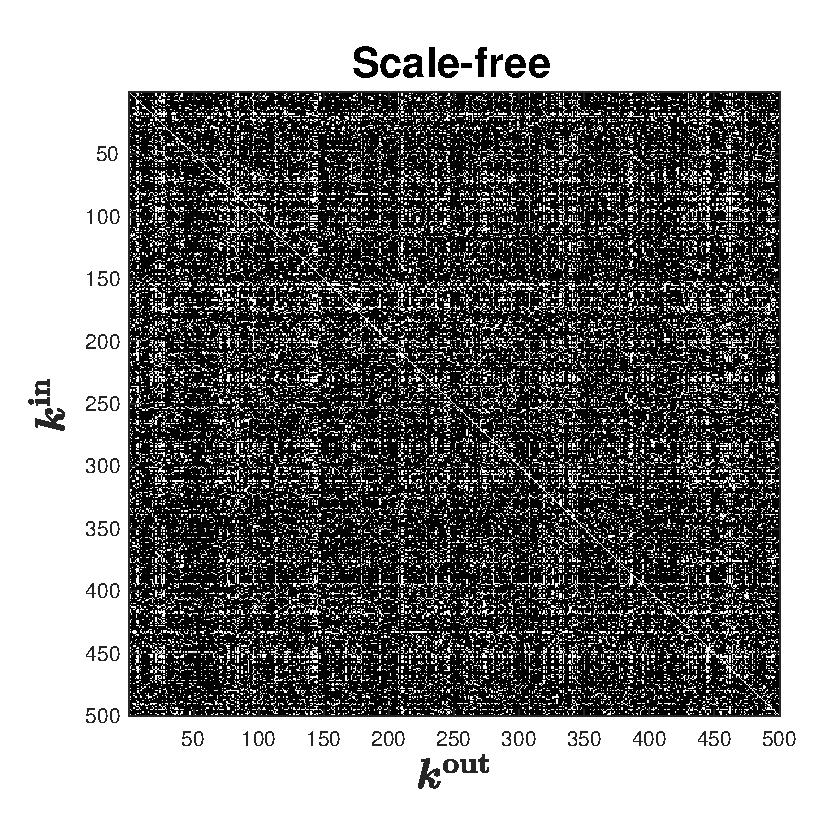
\includegraphics[width=\linewidth, trim={0.5cm 0.5cm 1cm 0.5cm },clip]{../Figures/Adjacency matrices/A_scalefree.pdf}
%   \caption{Adjacency matrix for a fixed-degree network.}
%   \label{fig:MFRCPW}
\end{subfigure}
   \caption{Adjacency matrices for different types of networks with $N$ = 500 and $\kmean$ = 100. We can see how the fixed-degree network is quite homogeneous, while the random network shows some more clustering. The scale-free network has a low number of nodes with a very high degree, which is why we see vertical and horizontal stripes in the adjacency matrix.}
   \label{fig:adjacencymatrices}
\end{figure}


\subsection{Initial conditions} \label{sec:initialconditions}
As the systems in \cref{eq:orderparameter,eq:OttAntonsenMeanField,eq:MeanField} describe the same dynamics for fully connected networks, it is important to be able to transform initial conditions between systems. If we expect their behaviour to be the same, then we need to test that by starting from the same point in time. Hence we can test whether \textsl{macroscopically} we can find the same equilibria, but we can also test \textsl{microscopically} whether the systems arrive at those points at the same time. 

%  If the initial conditions of all systems are exactly the same, then we should find that they describe the exact same behaviour.
% - macroscopically and microscopically - and this is the best way to test the \MFR theory. 

%When transforming between $\theta_i(t) \leftrightarrow z(\k,t) \leftrightarrow Z(t)$ we go from $\T^N \leftrightarrow \C^{M_\k} \leftrightarrow \C$. If we have the same initial conditions, then all systems will predict the same behaviour. We will only map everything to $\C$.\\
As we can only really study behaviour of $Z$ and $\overline{Z}$ in the complex unit circle, the most important relation we need to find is the transformation from $\C$ to $\T^{N}$ and from $\C$ to $\C^{M_{\k}}$, which yield the phase angles $\theta(0)_i$ and the degree dynamics $z(\k,0)$ from $Z(0)$ and $\overline{Z}(0)$ respectively. \\
% The following maps can be used to transform the initial conditions, but as they do not give any qualitative information on the dynamics or distributions of the variables, they are not valid for transforming between dynamics. \\

Let us start with the simplest transformation. Given an initial phase angle $\theta(0)_i$ or initial degree dynamics $z(\k, 0)$ we wish to find their resulting description in the complex unit circle. Mapping operations onto the order parameter is straightforward using \eqref{eq:orderparameter} and \eqref{eq:OttAntonsenMeanField}:
\begin{align}
\theta(0)_i \xrightarrow{\hspace*{8mm}} Z(0) &= \frac{1}{N} \sum_{j=1}^N e^{\ic\theta(0)_j} \label{eq:thetatoZ}\\
z(\k,0) \longrightarrow \overline{Z}(0) &= \frac{1}{N} \sum_{\k \in \K} P(\k) z(\k, 0)  \label{eq:ztoZ}
\end{align}
Starting from an initial synchronization $Z(0)$ and taking the inverse tranfsormation, we can make use of the fact that the average of a set of identical values is the value itself. This is simple for $\theta(0)_i$: we can take all phase angles to be the same at $t = 0$. For $z(\k,0)$ we have a weighed average which we need to undo, making sure that the whole sums up to $N$.
\begin{align}
Z(0) \xrightarrow{\hspace*{9mm}} \theta(0)_{i} &= -\ic \cdot \log \left( Z(0) \right)  \label{eq:Ztotheta} \\
Z(0) \longrightarrow z(\k,0) &= \frac{Z(0) \cdot n(\k)}{P(\k)} \label{eq:Ztoz}
\end{align}

Then, transforming between $\theta_i$ and $z(\k)$, we need to filter $\theta_i$ per degree as there exists usually more than one node with $\degree ( \theta_i ) = \k$:
\begin{alignat}{2}
z(\k,0) \longrightarrow \theta(0)_i &= -\ic \cdot \log \left( \frac{z(\k)\cdot P(\k)}{n(\k)} \right) \qquad \forall \: \theta \in \{ \theta \: | \: \degree(\theta) = \k \}  \label{eq:ztottheta}\\
\theta(0)_i \longrightarrow z(\k,0) &= \sum_{\k} e^{\ic \vartheta_{\k}} \qquad \qquad \vartheta_{\k} = \sum^{n(\k)} \theta \in  \label{eq:thetatoz}
\left\{ \theta \: | \: \degree(\theta) = \k \right\}
\end{alignat}
We can see how $\lim_{N \rightarrow +\infty} n(\k) = P(\k)$, which makes these maps exact for any network size. 


\subsection{Commutativity of complex vectors} 
It is important to notice that in \eqref{eq:OttAntonsenSystemFull} and \eqref{eq:OttAntonsenMeanField} and many other equations in this work, we compute an inner vector product, which is non-commutative for complex numbers:
\begin{align}
a \cdot b = \overline{b \cdot a} \qquad a, b \in \C^r
\end{align}
This is the result of the \textsl{Conjugate} or \textsl{Hermitian} symmetry of the inner product. This is especially important in the \matlab implementation, as one needs to remain consistent with left-hand or right-hand products.


\subsection{Fixed-degree networks as a baseline}
\begin{figure}[ht]
\centering
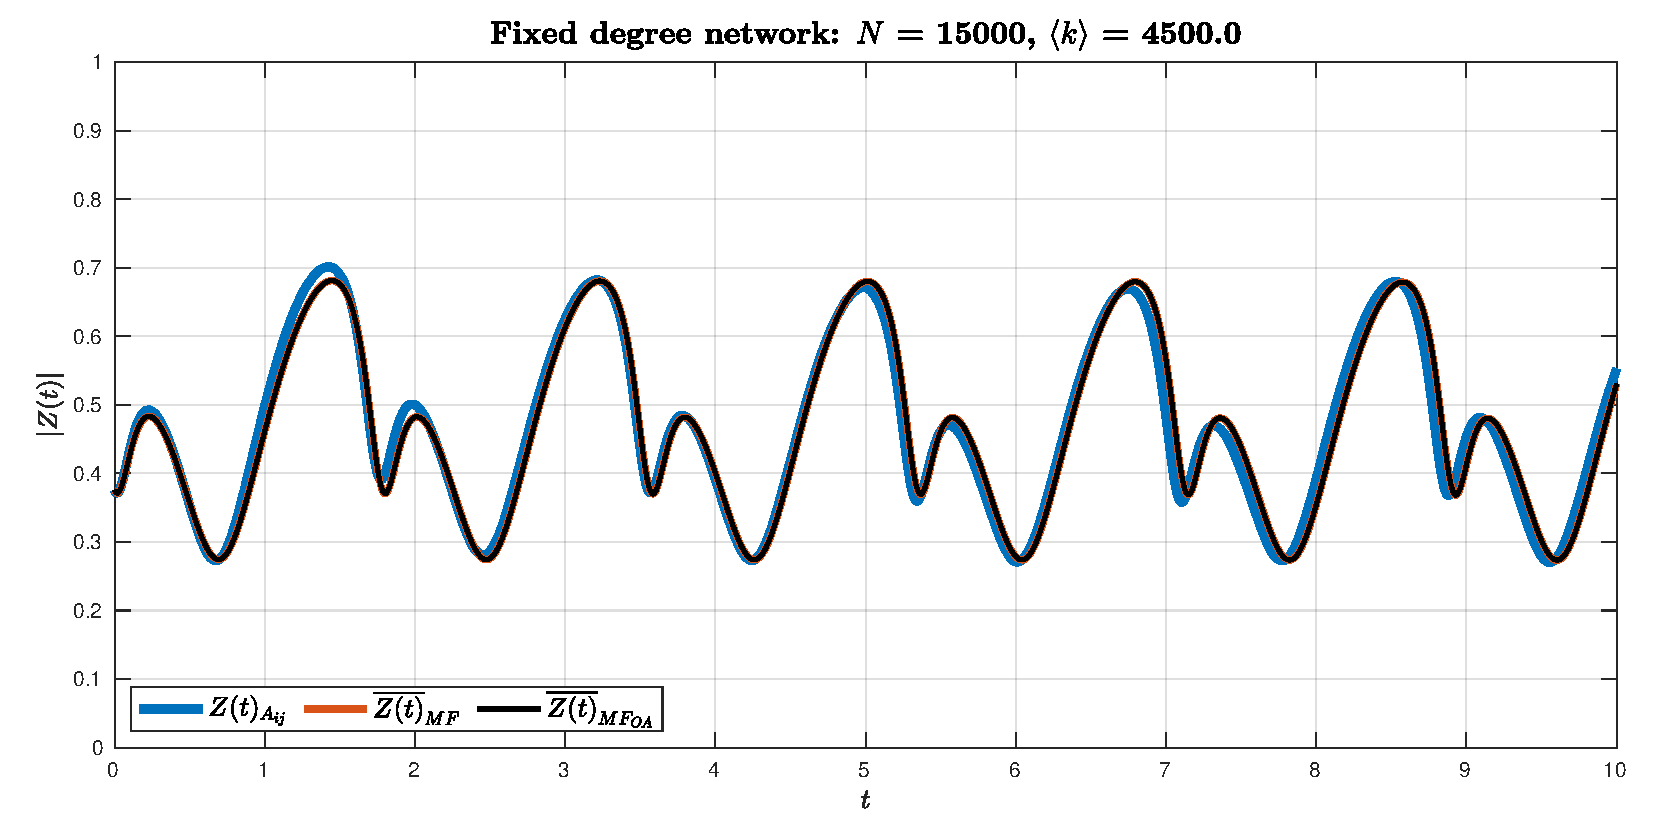
\includegraphics[width = \textwidth]{../Figures/InspectMeanFieldFixedDegree.pdf}
\caption{Comparison of the simulation of a fixed-degree network of Theta neurons and the Ott-Antonsen theory by the magnitude of the order parameter. We see that the same three macroscopic states are found by the three descriptions. As a matter of fact, the systems \eqref{eq:OttAntonsenMeanField} and \eqref{eq:MeanField} yield the exact same behaviour. There are small differences between simulation and theory, but these are most likely due to a finite network size and a finite integration step. This test benchmarks the lowest amount of error we can observe between simulation and theory, as for fixed-degree networks \eqref{eq:OttAntonsenSystemFull} consists of a single equation.}
\label{fig:InspectMeanFieldFixedDegree}
\end{figure}


\subsection{Fixed-degree networks as a baseline}

